\chapter{Outline of Approach}

\section{System Overview}

In order to demonstrate various performance engineering practices in the context of microservice design patterns, we look at a simple movie ticket reservation system, consisting of 3 independent cinemas (Cineworld \footnote{\url{https://www.cineworld.ie/}}, Dundrum \footnote{\url{https://www.movies-at.ie/movies/}} and UCD \footnote{\url{https://www.ucd.ie/studentcentre/cinema/}}), as well as an intermediary (or broker) between clients and the cinema services. Each cinema has its own catalogue of movies (with an ID, name, and available showtimes). The client's primary objective would be to request the intermediary to fetch a list of movies from every active cinema, then display aggregated results. Next, the client selects a movie and showtime (along with other booking details) to make a reservation at a specific cinema. It is also possible to list the reservations made at a given cinema (useful for staff and administrators). The intermediary serves as a router for client requests to the cinema services, and in some cases, an aggregator of results.


\begin{figure}[H]
  \centering
  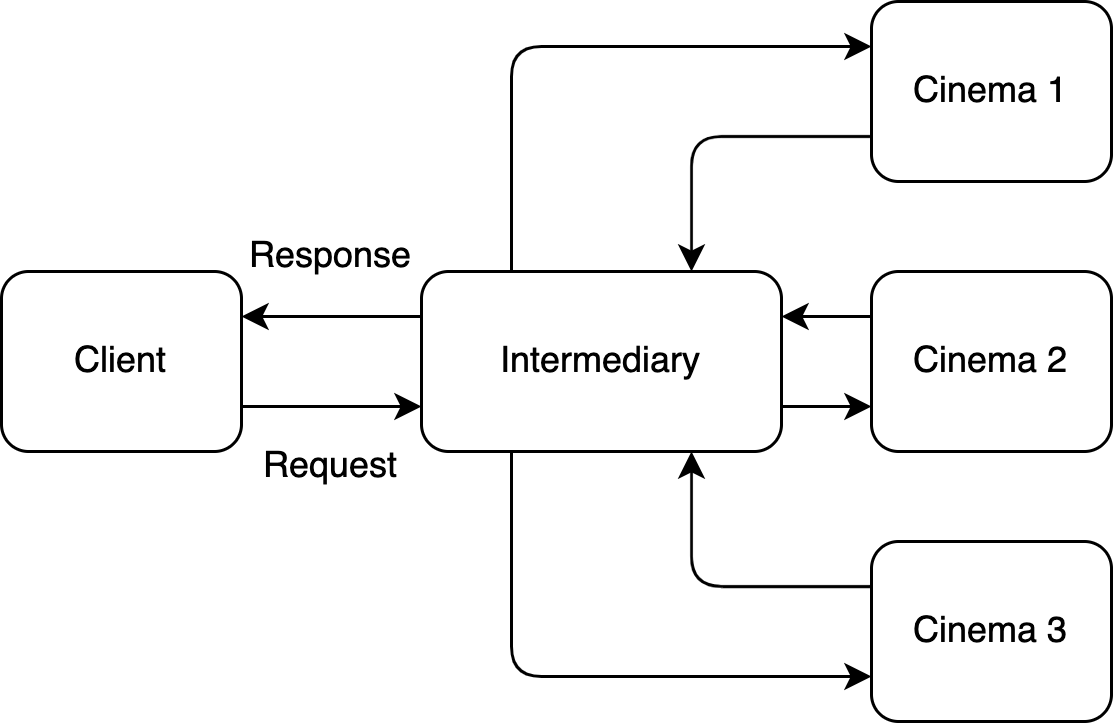
\includegraphics[width=0.5\linewidth]{./assets/diagrams/outline-arch.png}
  \caption{Prototype of movie ticket reservation system using microservices.}
  \label{fig:outline-arch}
\end{figure}

\section{Case Studies}

In this project, two separate web applications have been designed to model the same system described above, each employing a variety of common design patterns. The applications follow microservice architecture, with the intermediary and cinema services all being self-contained, loosely-coupled and independently deployable. Taking each application to be a \textit{case study}, the next chapter provides descriptions of the system design, implementation specifics, design pattern choices, and the associated performance implications. In a larger scale production system, it is likely that each independent cinema would in turn comprise a number of microservices to serve more specific purposes, but to avoid over-complicating the architecture in this project, cinemas are designed to be single entities.

\subsection{Communication Styles}

When migrating from monolithic applications to microservices, decisions regarding communication mechanisms are vital, since a number of internal services must efficiently interact with each other as well as the clients, in order to perform well in a distributed environment. Managing data from responses, and aggregating results from various services also becomes a part of the equation. The two case studies in this project illustrate the two most common communication style patterns, namely HTTP \footnote{\url{https://developer.mozilla.org/en-US/docs/Web/HTTP}} request/response using APIs (typically RESTful \footnote{\url{https://en.wikipedia.org/wiki/Representational_state_transfer}}) in case study 1, and asynchronous messaging following a protocol like AMQP \footnote{\url{https://en.wikipedia.org/wiki/Advanced_Message_Queuing_Protocol}} in case study 2. Broadly speaking, the first style uses a synchronous protocol (HTTP), where the client awaits a response from services after sending a request. Then, as the name suggests, the second style uses an asynchronous protocol (AMQP) that uses message queues, and doesn't wait for responses. These have been separated from demonstration, but in practice, microservice-based applications tend to employ a combination of synchronous and asynchronous communication styles (including deferred synchronous and asynchronous callbacks) depending on the use case. Microservices often face the issue of "chattiness", due to excessive inter-service communication leading to performance degradation, which is a point to keep in mind when developing microservices. The aim is to enforce the autonomy of microservices during integration, and avoid anti-patterns such as a distributed monolith, where services end up being tightly coupled.

\subsection{Choice of Tools}

One of the main benefits of microservices is the freedom of choice regarding the programming language used for development, since any suitable language may be used as long the service exposes an API \footnote{\url{https://www.mulesoft.com/resources/api/what-is-an-api}} adhering to known standards (typically HTTP and REST). The API is then used for inter-service communication. For the case studies in this project, Java and Spring \footnote{\url{https://spring.io}} are chosen over other languages and frameworks primarily due to the dominance of Java in enterprise-level software, as well as the feature richness of Spring. Moreover, as shown in a 2017 study by Pereira et al. \cite{pereira17}, Java ranks much higher in terms of time, memory and energy efficiency; which need to be considered when talking about system performance; compared to other popular languages such as Python or TypeScript/JavaScript. The Spring framework in Java offers a plethora of integrations and abstractions to implement microservice and cloud-related design patterns, through projects such as Spring Boot, Spring Data, Spring Cloud and Spring AMQP, to name a few that are used in the case study web applications here. Apache Maven \footnote{\url{https://maven.apache.org}} is the tool used for dependency management for Java.

Each web application exposes APIs for its microservices, whose endpoints can be invoked with HTTP requests like GET and POST. In commercial systems, a website (UI client) would invoke the backend API to perform actions, but for our case studies, it is sufficient to use a tool such as Postman \footnote{\url{https://www.postman.com}} or VS Code's REST Client \footnote{\url{https://marketplace.visualstudio.com/items?itemName=humao.rest-client}} to demonstrate the API functionalities locally.

\section{Deployment}

In line with industry standards, Docker \footnote{\url{https://www.docker.com}} is the infrastructure/containerisation tool used to deploy the fleet of microservices. According to Docker, Inc., a \textit{container image} is a lightweight, standalone, executable package of software that includes everything needed to run an application: code, runtime, system tools, system libraries and settings. Using Docker provides a number of advantages such as ease of standardisation, compatibility, maintainability, CI/CD, resource and application isolation, and much more. Container deployment and application testing is performed on an Ubuntu 18.04 LTS compute server (\textit{dunnion}, maintained by the UCD School of Computer Science \footnote{\url{https://www.ucd.ie/cs/}}), with a 10 core Intel(R) Xeon(R) Silver 4114 CPU (base frequency: 2.20 GHz), and 125GB system memory.

\section{Evaluation}